\documentclass[12pt,journal,a4paper,twocolumn,final,oneside]{IEEEtran}%final,finalsubmission,

\usepackage{multicol}

\usepackage{color}

\usepackage{subfigure}

 \usepackage[plainpages=false,pdfpagelabels,breaklinks=true,pdfborder=0 0 0]{hyperref} % pagebackref

% \def\pagedeclaration#1{\dotfill\nobreakspace\hyperpage{#1}}
% \def\nomentryend{}
% \def\nomlabel#1{\textbf{#1}\hfil}
% \newcommand*{\eqdeclaration}[1]{%
%   \hyperlink{equation.#1}{(Equation~#1)}%
% }
%
% \renewcommand{\backref}[1]{}
% \renewcommand*{\backrefalt}[4]{%
%   \ifcase #1 %
%     %
%   \or
%     \ \emph{(cited on page #2)}.%
%   \else
%     \ \emph{(cited on pages #2)}.%
%   \fi
% }

\usepackage{rotating}
\usepackage[sort,compress,numbers]{natbib} %round,authoryear


% %% BEGIN: Include label in list of references
% \makeatletter
% \def\mysplit#1)#2\@nil{%
% \def\@mysecondoftwo{#2}%
% \ifthenelse{\equal{@@arg}{#1}}
% {% no year, take everything
% \def\@mycitep{#1}}
% {% take the part until and including year
% \def\mycitep{#1)}}}
%
% \def\@lbibitem[#1]#2{%
% \mysplit#1)@@arg\@nil
% \if\relax\@extra@b@citeb\relax\else
% \@ifundefined{br@#2\@extra@b@citeb}{}{%
% \@namedef{br@#2}{\@nameuse{br@#2\@extra@b@citeb}}}\fi
% \@ifundefined{b@#2\@extra@b@citeb}{\def\NAT@num{}}{\NAT@parse{#2}}%
% \item[\hfil\hyper@natanchorstart{#2\@extra@b@citeb}{[{\mycitep}]}%
% \hyper@natanchorend]%
% \NAT@ifcmd#1(@)(@)\@nil{#2}}
% \makeatother
% % %% END: Include label in list of references

\usepackage{nomencl}
\def\nomname{Glossary}
\makenomenclature

\usepackage{graphicx}

% correct bad hyphenation here
\hyphenation{op-tical net-works semi-conduc-tor SPECjAppServer experi-ments}

% \newcommand{\TODO}[1]{\textcolor{red}{\footnote{\textcolor{red}{#1}}}\marginpar{\textcolor{red}{\scriptsize{TODO}}}}
% \newcommand{\MR}[1]{\textcolor{red}{\footnote{\textcolor{red}{#1}}}\marginpar{\textcolor{red}{\scriptsize{Matthias}}}}
% \newcommand{\WH}[1]{\textcolor{red}{\footnote{\textcolor{red}{#1}}}\marginpar{\textcolor{red}{\scriptsize{Willi}}}}
% \newcommand{\JW}[1]{\textcolor{red}{\footnote{\textcolor{red}{#1}}}\marginpar{\textcolor{red}{\scriptsize{Jan}}}}
% \newcommand{\SF}[1]{\textcolor{red}{\footnote{\textcolor{red}{#1}}}\marginpar{\textcolor{red}{\scriptsize{S\"{o}ren}}}}
% \newcommand{\TODOBOX}[1]{\qquad\newline\fbox{\fbox{\parbox{0.95\columnwidth}{\textbf{\color{red}{%TODO:
% }}\noindent  #1 }}\\[0.1cm]}\marginpar{\textcolor{red}{\scriptsize{TODO}}}}

\usepackage{tipa}
\newcommand{\SLAstic}{\mbox{SLAstic}}
\newcommand{\SLAsticPhonetic}{{\sffamily\mbox{SLAstic}}}
\newcommand{\SLAsticComponent}[1]{\mbox{SLAstic.#1}}
\newcommand{\SLAsticSIM}{\SLAsticComponent{SIM}}
\newcommand{\SLAsticMON}{\SLAsticComponent{MON}}
\newcommand{\SLAsticREC}{\SLAsticComponent{REC}}
\newcommand{\SLAsticCTRL}{\SLAsticComponent{CONTROL}}

%Allow more images on one page
\renewcommand\floatpagefraction{.9}
\renewcommand\topfraction{.9}
\renewcommand\bottomfraction{.9}
\renewcommand\textfraction{.1}   
\setcounter{totalnumber}{50}
\setcounter{topnumber}{50}
\setcounter{bottomnumber}{50}

% \newcommand{\filename}[1]{\textit{\texttt{\small #1}}}
\newcommand{\opname}[1]{\textit{#1}}
% \newcommand{\opnamesmaller}[1]{\textit{\texttt{\scriptsize #1}}}

\newcommand{\classname}[1]{\textit{#1}}
% \newcommand{\pkgname}[1]{\textit{\texttt{\small #1}}}
\def\@hyph{\hbox{$\hookleftarrow$}} \def\+{\discretionary{\@hyph}{}{}}

\urlstyle{same}
% \usepackage{color}
% \definecolor{mygray}{gray}{.75}
\usepackage{listings}
\lstset{%
        language=JAVA,
        basicstyle=\scriptsize, %\footnotesize,
        identifierstyle={},
        commentstyle=\itshape,
        stringstyle=\emph,
        keywordstyle=\ttfamily,
        numbers=left,
        stepnumber=1,
        tabsize=2,
        numbersep=6.5pt,
        xleftmargin=13pt,
        xrightmargin=10pt,
%        numberstyle=\tiny,
%%        numberblanklines=false,
         frame=single,
%         backgroundcolor=\color{mygray},
        breaklines=true,
%        captionpos=t,
        mathescape=true,
        showspaces=false,
        showtabs=false,
%        columns=spaceflexible,
}
%% Listings Fix for IEEETran (only caption, title still doesn't work!)
\makeatletter
\def\lst@makecaption#1#2{\@makecaption{#1}{#2}{}}
\makeatother

\usepackage{pdfpages}

\begin{document}

%\includepdf[nup=1x1,pages=-]{TRTitelA4-p1}

\setcounter{page}{1}

\title{%
Kieker Architecture%
}

\author{%
Kieker team
}

\maketitle

\begin{abstract}\small
\ldots
\end{abstract}

\section{Framework Architecture} 
\newcommand{\KiekerTerminology}[1]{{\small\sffamily #1}}
\newcommand{\MonitoringProbe}{\KiekerTerminology{Monitoring Probe}}
\newcommand{\MonitoringProbes}{\KiekerTerminology{Monitoring Probes}}
\newcommand{\MonitoringLog}{\KiekerTerminology{Monitoring Log}}
\newcommand{\MonitoringLogWriter}{\KiekerTerminology{Monitoring Log Writer}}
\newcommand{\MonitoringLogWriters}{\KiekerTerminology{Monitoring Log Writers}}
\newcommand{\MonitoringLogReader}{\KiekerTerminology{Monitoring Log Reader}}
\newcommand{\MonitoringLogReaders}{\KiekerTerminology{Monitoring Log Readers}}
\newcommand{\MonitoringRecord}{\KiekerTerminology{Monitoring Record}}
\newcommand{\MonitoringRecords}{\KiekerTerminology{Monitoring Records}}
\newcommand{\MonitoringRecordConsumer}{\KiekerTerminology{Monitoring Record Consumer}}
\newcommand{\MonitoringRecordConsumers}{\KiekerTerminology{Monitoring Record Consumers}}
\newcommand{\KiekerTpmon}{\KiekerTerminology{Kieker.Tpmon}}
\newcommand{\KiekerTpan}{\KiekerTerminology{Kieker.Tpan}}
\newcommand{\TpmonController}{\KiekerTerminology{TpmonController}}
\newcommand{\TpanInstance}{\KiekerTerminology{TpanInstance}}

\noindent This section provides an overview of Kieker's framework
architecture.
The outstanding features of Kieker may be summarized as follows:
 \begin{itemize}
 \item A common, extensible monitoring record model that is shared among the logging and analysis component: in this paper, we use record types for storing response times (in this section), %
 and (distributed) trace information~(Sections~\ref{sec:tracing} and~\ref{sec:casestudy}). % we could also record resource utilization data or other system information that is measurable.
 \item An extensible reader/writer model: the monitoring records may be written to and being read from relational databases, to the file~system or to JMS queues; additional data sinks may be added.
\pagebreak
 \item An extensible monitoring record consumer model: the monitoring records may be analyzed and visualized for various purposes.  If the monitoring log is based on a messaging middleware, continuous online analysis is supported.
 \end{itemize}
 
\noindent The Unified Modeling Language~(UML)~%
\citep{OMG2007UML22Superstructure} is employed for describing the architecture, independent of the programming language (which is Java for Kieker).

\begin{figure}\centering
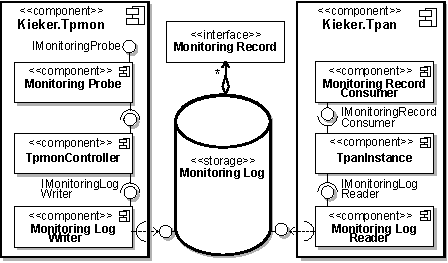
\includegraphics[width=1\columnwidth]{figures/kiekerComponentDiagram-woCloud-bw}%
\caption{Top-level view on Kieker's architecture}
\label{fig:kieker:coreFrameworkComponents}
\end{figure}

At the top-level, Kieker is partitioned into the two components \KiekerTpmon{} and %
\KiekerTpan{} with the \MonitoringLog{} in between, as illustrated in Figure~\ref{fig:kieker:coreFrameworkComponents}. %
\KiekerTpmon{} provides a reusable infrastructure for collecting %
application-level monitoring data in \MonitoringProbes{} and writing this %
monitoring data to the \MonitoringLog{}, e.g., the local file system, a database, or %
a messaging queue, using a \MonitoringLogWriter{}. %
The \TpmonController{} %
is responsible for initializing and controlling a \KiekerTpmon{} instance. %
The \MonitoringLog{} contains \MonitoringRecords{}, as defined in Figure~%
\ref{fig:kieker:coreFrameworkComponents}. %TR: \ref{fig:kieker:coreFrameworkClassesAndInterfaces:record}. 
Each record holds the %
monitoring data of a single measurement created by the \MonitoringProbes{}. %
\KiekerTpan{} provides the infrastructure for analyzing the \MonitoringLog{}: %
a \MonitoringLogReader{}~(Figure~\ref{fig:kieker:coreFrameworkComponents}) reads \MonitoringRecords{} from the %
\MonitoringLog{} and delivers these to registered \MonitoringRecordConsumers{}, according to the observer design pattern~\citep{GammaHelmJohnsonVlissides1995DesignPatternsElementsOfReusableObjectOrientedSoftware}. %
\MonitoringRecordConsumers{} perform the actual analysis or visualization functionality. %
A \KiekerTpan{} instance is initialized and controlled by a \TpanInstance{} %
instance (Figure~\ref{fig:kieker:coreFrameworkComponents}). %

\begin{figure}
\centering
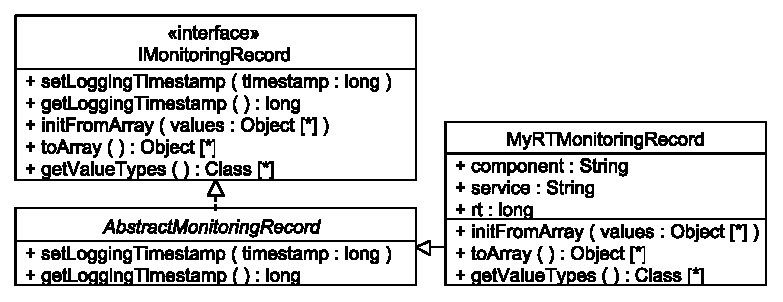
\includegraphics[scale=0.65]{figures/model/kieker_MyRTMonitoringRecord}%
% TR: \includegraphics[width=0.9\columnwidth]{figures/KiekerInterfaceOverviewReArranged-woMonitoringRecord-bw-record-withRTRecord}%
\caption{Monitoring Record interface and abstract class, as well as a concrete Monitoring Record as example.}
\label{fig:kieker:coreFrameworkClassesAndInterfaces:record}
\end{figure}

\begin{figure}\centering
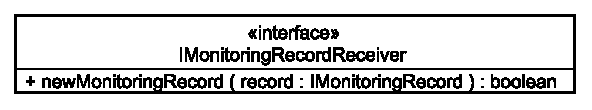
\includegraphics[scale=0.65]{figures/model/kieker_IMonitoringRecordReceiver}
\caption{Monitoring Record Receiver}
\label{fig:record:IMonitoringRecordReceiver}
\end{figure}

\begin{figure}\centering
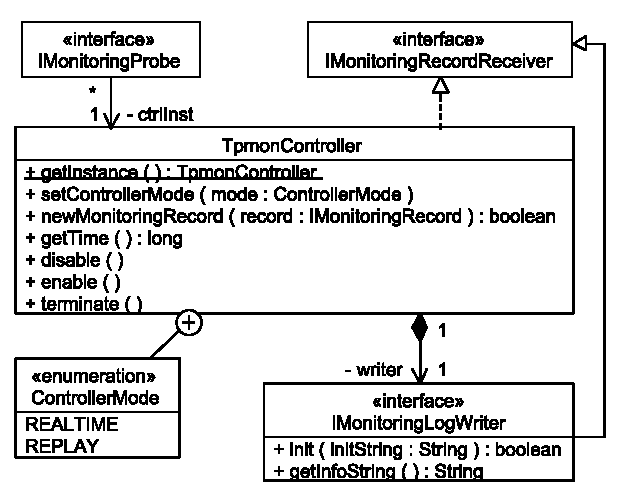
\includegraphics[scale=0.65]{figures/model/kieker_TpmonController}% 
% TR: \includegraphics[scale=0.69]{figures/KiekerInterfaceOverviewReArranged-woMonitoringRecord-bw-tpmon}%
\caption{Kieker.Tpmon}
\label{fig:kieker:coreFrameworkClassesAndInterfaces:tpmon}
\end{figure}

\begin{figure}\centering
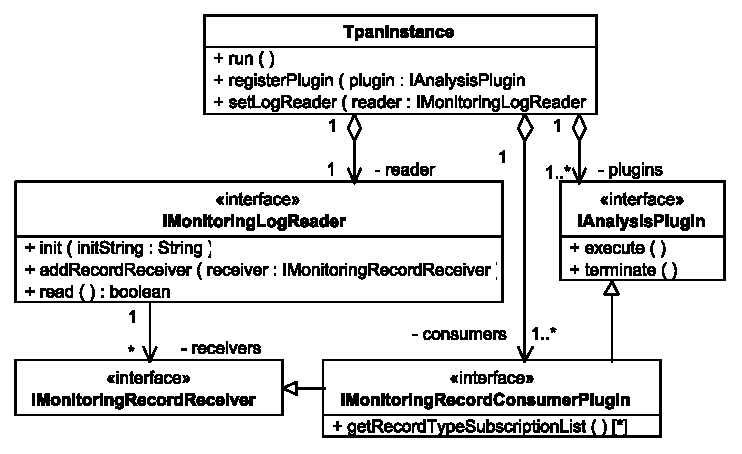
\includegraphics[scale=0.65]{figures/model/kieker_TpanInstance}%
% TR: \includegraphics[scale=0.69]{figures/KiekerInterfaceOverviewReArranged-woMonitoringRecord-bw-tpan}%
\caption{Kieker.Tpan}
\label{fig:kieker:coreFrameworkClassesAndInterfaces:tpan}
\end{figure}

\begin{figure*}\centering
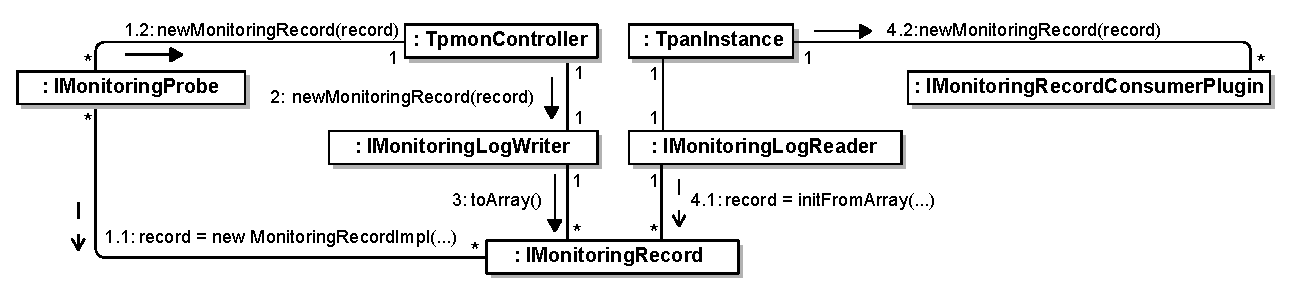
\includegraphics[width=0.8\textwidth]{figures/kiekerCommunications-revisedReArranged-woMonitoringLog-bw}%
\caption{Communication among framework components %
%{\textcolor{red}{S\"{o}ren: Evtl. spezifischer angeben, welche Kommunikation gezeigt wird? Im Text ist vom Life-Cycle eines Monitoring-Records die Rede}}
for creating and writing a Monitoring Record in Kieker.Tpmon~(1.1--3) as well as %
reading and using this Monitoring~Record in Kieker.Tpan~(4.1,~4.2). %
}
\label{fig:kieker:communicationsAmongCoreFrameworkComponents}
\end{figure*}

Figure~\ref{fig:kieker:coreFrameworkClassesAndInterfaces} shows the core
% \WH{etwas Erl\"{a}uterung zu den Assoziationen?}
% Anm. Andr\'{e}: Ja, hier koennte man noch mehr erklaeren ...
Kieker framework classes and interfaces with their associations in a UML~Class %
Diagram notation. %
Kieker offers different implementations for the \MonitoringRecord{}, %
\MonitoringProbe{}, \MonitoringLogWriter{}, %
\MonitoringLogReader{}, and \MonitoringRecordConsumer{} %
components and allows to use customized components created by implementing or %
extending the interfaces or abstract classes of the framework corresponding to these components, as described below.
% 
% % \newpage
% 
Figure~\ref{fig:kieker:communicationsAmongCoreFrameworkComponents} illustrates a \MonitoringRecord{}'s life cycle. It shows the
sequence of interactions among instances of the
Kieker components in a UML~Communication Diagram
notation, whereby the numbers at the operation calls, which are attached to the links, define the order. The multiplicities at the links indicate the possible number of these links among respective object instances.


% \subsection{Framework Components}

% A singleton~%
% \cite{GammaHelmJohnsonVlissides1995DesignPatternsElementsOfReusableObjectOrientedSoftware} %
% instance of t

% \newpage

\subsection{Monitoring Record}\label{sec:architecture:record}

\noindent A \MonitoringRecord{} holds the measurement data collected in a single measurement. %
Different types of \MonitoringRecords{} can be used together in one \KiekerTpmon{} %
instance. %
Figure~\ref{fig:kieker:coreFrameworkClassesAndInterfaces:record} shows a %
concrete \MonitoringRecord{} type \classname{MyRTMonitoringRecord} which can be used %
to store response times of services provided by software components. %
As required by all \MonitoringRecord{} types, it implements the interface \classname{IMonitoringRecord}---%
in this case by extending the abstract framework class \classname{Abstract\+MonitoringRecord}. %

\subsection{Monitoring Probe}\label{sec:monitoringProbe}
% 
% % \begin{figure}
% % % \begin{minipage}[t]{0.4\textwidth}
% %  \begin{multicols}{2}
% % \parbox{0.45\textwidth}{
% % \subfigure[Probe package]{\label{fig:probePackage}%
% % \includegraphics[width=0.4\textwidth]{figures/monitoringProbe}%
% % }\\\quad\\
% % }\newpage
% % % \end{minipage}
% %
% % \subfigure[Example AspectJ response time probe]{%
% % \includegraphics[width=0.46\textwidth]{figures/probe-example}%
% % }
% % \end{multicols}
% % \caption{TODO}
% % \end{figure}
% 
\noindent A \MonitoringProbe{} (Figure~\ref{fig:kieker:coreFrameworkComponents}) contains the measurement logic which collects and possibly %
pre-processes measurement data from the application. %
A \MonitoringProbe{} creates an instance of a \MonitoringRecord{} and sends this %
\MonitoringRecord{} to the \TpmonController{} by calling the
method \opname{newMonitoringRecord(..)} of the \TpmonController{}, as shown in %
Figure~\ref{fig:kieker:communicationsAmongCoreFrameworkComponents}. %Abstract\+Kieker\+MonitoringRecord record)}. %
All \MonitoringProbe{} types must implement the interface \classname{IMonitoring\+Probe} (Figure~\ref{fig:kieker:coreFrameworkClassesAndInterfaces}). %

\MonitoringProbes{} of different types can be used together in a single \KiekerTpmon{} %
instance and are typically tightly bound to middleware underlying the application. %
% The location of a monitoring probe within an instrumented system is called a %
% \textit{monitoring point}.
For example, the interception APIs of Java middleware technologies provided by the
Spring framework, the Java Servlet specification, and the Apache~CXF Web service
framework can be used to implement and integrate \MonitoringProbes{} into an application. %
In Section~\ref{sec:casestudy}, we demonstrate how different technology-specific
types of \MonitoringProbes{} can be used in combination to monitor distributed traces.

% \begin{minipage}{\columnwidth}
\begin{lstlisting}[float, language=Java, caption=Example AspectJ response time Monitoring Probe, label=lst:aspectJRTMonitoringProbe]
@Aspect
public class MyRTMonitoringProbe
       implements IMonitoringProbe {

 static final TpmonController CTRL =
        TpmonController.getInstance();

 @Around
    (value="execution(@MyRTProbe * *.*(..))")
 public Object probe(ProceedingJoinPoint j)
        throws Throwable {
  MyRTMonitoringRecord record =
                new MyRTMonitoringRecord();
  record.component = j.getSignature()
                      .getDeclaringTypeName();
  record.service = j.getSignature().getName();
  Object retval;
  long tin = CTRL.getTime();
  try { retval = j.proceed(); }
  catch (Exception e) { throw e; }
  finally {
   record.rt = CTRL.getTime() - tin;
   CTRL.newMonitoringRecord(record);
  }
  return retval;
 }
}
\end{lstlisting}
% \end{minipage}

As an example, Listing~\ref{lst:aspectJRTMonitoringProbe} shows an AspectJ-based \MonitoringProbe{} %
which measures response times of Java methods and stores this data as \MonitoringRecords{} %
of the previously introduced type \classname{MyRTMonitoringRecord} (Figure~\ref{fig:kieker:coreFrameworkClassesAndInterfaces:record}). %
In this example, all Java methods annotated with \classname{MyRTProbe} %
are instrumented, as follows for the method \classname{searchBook()} via Java annotation:\\

\begin{minipage}{\columnwidth}
{\small
\begin{verbatim}
@MyRTProbe()
public static void searchBook() { .. }
\end{verbatim}
}
\end{minipage}\\

% Integration into application code:
% \begin{itemize}
% \item Java annotations/AOP (AspectJ)
% \item Interception APIs (Spring, Servlet, CXF)
% \item Manual integration (facade pattern)
% \end{itemize}

% \WH{Gewisse Erl\"{a}uterung zu Listing~\ref{lst:aspectJRTMonitoringProbe} n\"{o}tig}

\noindent Calls to an instrumented method are intercepted and the execution %
proceeds with the method \classname{probe(..)}~(lines~10--26) containing the %
response time measurement logic of the \MonitoringProbe{}. %
Before the execution is delegated to the intercepted method~(line~19), %
a \MonitoringRecord{} instance is created and initialized~(lines~13--16) %
and the timestamp before the execution is taken~(line~18). %
After this execution returns, the response time is calculated and stored in %
the \MonitoringRecord{}~(line~22) which is then passed to the \TpmonController{} %
instance~(line~23).

\subsection{Monitoring Log Writer}\label{sec:monitoringlogwriter}

\begin{figure}\centering
\subfigure[Implemented writers]{\label{fig:writers}%
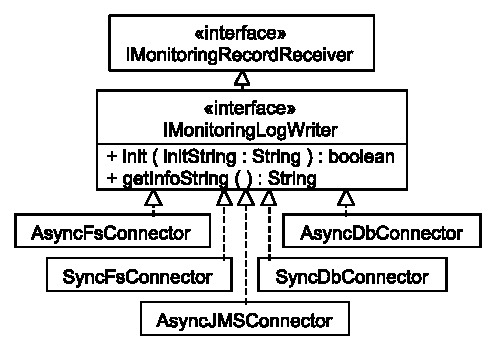
\includegraphics[scale=0.65]{figures/model/kieker_writerimpls}%
% TR: \includegraphics[scale=0.8]{figures/tpmon-writers-refined-bw}%
}\qquad
\subfigure[Implemented readers]{\label{fig:readers}%
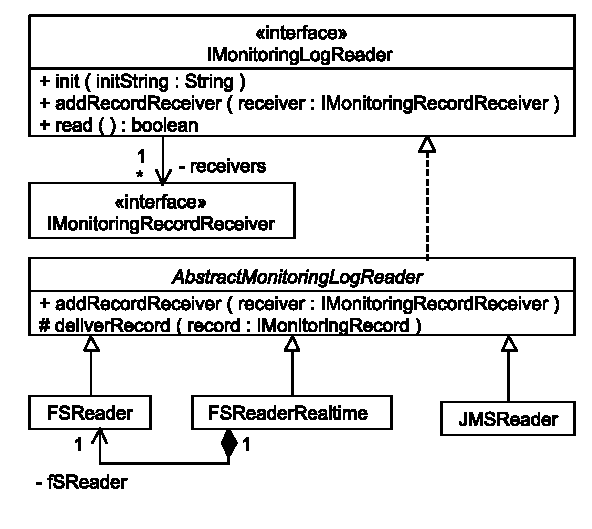
\includegraphics[scale=0.65]{figures/model/kieker_readerimpls}%
%TR: \includegraphics[scale=0.8]{figures/tpmon-readers-refined-bw}%
}
\caption{Implemented monitoring log writers and readers. %The abstract classes have been introduced in Figure~\ref{fig:kieker:coreFrameworkClassesAndInterfaces}.
}
\label{fig:writersAndReader}
\end{figure}

\noindent A \MonitoringLogWriter{} is responsible for writing/serializing the %
\MonitoringRecords{} to the \MonitoringLog{}. %
For each \MonitoringRecord{} to be logged, the writer is invoked
by the \TpmonController{} and writes the data contained in the retrieved \MonitoringRecord{} %
by calling the \MonitoringRecord{}'s \classname{toArray()} method, %
as illustrated in Figure~\ref{fig:kieker:communicationsAmongCoreFrameworkComponents}. %
% A \classname{TpmonController} initializes and uses exactly one monitoring log writer.
Figure~\ref{fig:writers} shows the \MonitoringLogWriters{} which are already included %
in the Kieker framework, supporting the file system, relational databases, and JMS %message
queues. %
The prefixes \textit{Sync/Async} in Figure~\ref{fig:writers} indicate whether the I/O operation required to %
log the \MonitoringRecord{} is performed within the \MonitoringProbe{}'s thread of control~%
(synchronously) or by one or more asynchronous writer thread(s) using an internal buffer. %
The filesystem writer stores \MonitoringRecords{} represented as comma-separated values~(CSV). %
Listing~\ref{lst:RTMonitoringLog} shows a sample filesystem \MonitoringLog{} %
containing entries of the \classname{MyRTMonitoringRecord} \MonitoringRecord{} type. %
Each line contains the \MonitoringRecord{} type identifier, as well as the values
of the record fields \textit{loggingTimestamp}~(cropped in the listing), \textit{component}, \textit{service}, %
and \textit{rt}~(response time in nanoseconds). %
A mapping file is used to store the mapping between a \MonitoringRecord{} type %
identifier and its implementing class, as shown in Listing~\ref{lst:RTMonitoringLogMapping}. %
% %The mapping is required since \MonitoringRecords{} of different type are written to
% %the same file and to allow ...
% 
% % Monitoring log writers must extend the abstract class %
% % \classname{Abstract\+Kieker\+Monitoring\+Log\+Writer}. %
% 
% % \WH{Beispiel kurz erl\"{a}utern? Gut w\"{a}re es evtl ein zweites Record zu haben, damit Listing 4 mehr Sinn macht.}
% % Anm. Andr\'{e}: Ja, w\"{a}re gut ein zweites zu haben; z.B. das in Kieker enthaltene
% %             BranchingRecord, das man verwenden kann, um zu loggen, welche
% %             Ast einer Verzweigung genommen wird.
% %             Aus Zeitgr\"unden habe ich das jetzt nicht mehr gemacht.
\begin{minipage}{\columnwidth}
\begin{lstlisting}[language=Java, numbers=none, xleftmargin=0pt, caption=Filesystem Monitoring Log with Monitoring Records of type MyRTMonitoringRecord, label=lst:RTMonitoringLog, basicstyle=\ttfamily\footnotesize]
$\$$1;..267737726;Catalog;getBook;2104283
$\$$1;..268321753;Catalog;getBook;2679347
$\$$1;..324713919;Catalog;getBook;20082302
$\$$1;..324780416;CRM;getOffers;20164491
$\$$1;..324787610;Bookstore;searchBook;93795571
$\$$1;..325166071;Catalog;getBook;20568496
$\$$1;..325180972;CRM;getOffers;20612072
$\$$1;..325186824;Bookstore;searchBook;94195055
\end{lstlisting}

\begin{lstlisting}[language=Java, numbers=none, xleftmargin=0pt, caption=Mapping of Monitoring Record type identifier to implementing class, label=lst:RTMonitoringLogMapping, basicstyle=\ttfamily\small]
$\$$1=MyRTMonitoringRecord
\end{lstlisting}
\end{minipage}

\subsection{Monitoring Log Reader}

\noindent A \MonitoringLogReader{} is used to create \MonitoringRecord{} instances from %
a \MonitoringLog{} written by a corresponding \MonitoringLogWriter{} (by
calling a \MonitoringRecord{}'s \classname{init\+FromArray(..)} method), see Figure~\ref{fig:kieker:coreFrameworkClassesAndInterfaces:record}. %%
As shown in Figure~\ref{fig:readers}, %
% Monitoring log readers must extend the abstract class %
% \classname{Abstract\+Kieker\+Monitoring\+Log\+Reader}. %
Kieker includes \MonitoringLogReaders{} corresponding to the included writers %
for the filesystem and for JMS queues. %
% \WH{and databases ?}
% Anm. Andr\'{e}: Nein, einen DB-reader haben wir in dieser Implementierung zur Zeit noch nicht.  %
% A \classname{TpanInstance} instance uses exactly one monitoring log reader. %
\MonitoringLogReaders{} extend the abstract class \classname{Abstract\+Monitoring\+Log\+Reader}, %\classname{Abstract\+Kieker\+Monitoring\+Log\+Reader},
which already provides convenient functionality for handling the subscription of %
\MonitoringRecordConsumers{} to \MonitoringRecords{} of specific types as well as %
the delivery of records to the subscribers. %

% Monitoring log readers are also used to replay monitoring logs, e.g., in order
% to run analysis routines with . %
Additionally, Kieker includes the \MonitoringLogReader{} \classname{FSReaderRealtime} %
which can be used to replay \MonitoringRecords{} from a filesystem-based %
\MonitoringLog{} in the original timescale. This has proven to be very helpful for debugging purposes and for simulating %
continuously incoming monitoring data while developing online analysis components. %
% %
% 
\subsection{Monitoring Record Consumer}
% 
% \begin{figure}\centering
% % \subfigure[Kieker.Tpan class diagram]{%
% % \includegraphics[width=0.75\textwidth]{figures/LogAnalysisMetaModel}%
% % }
% % \subfigure[UML Communication Diagram]{%
% 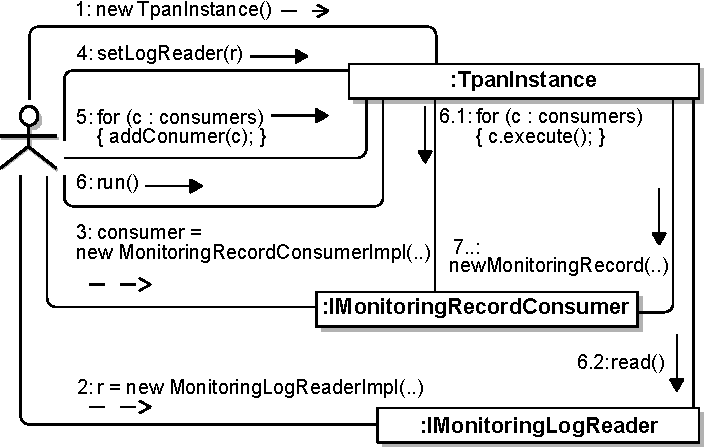
\includegraphics[width=\columnwidth]{figures/LogAnalysisCommunications-bw}%
% % }
% % \subfigure[Code example]{%
% % \includegraphics[width=0.35\textwidth]{figures/logAnalysis-ctrlExample}
% % }
% \caption{Kieker.Tpan communication diagram}
% \label{fig:tpanCommunicationDiagram}
% \end{figure}
% 
\noindent Analysis or visualization components are integrated into \KiekerTpan{} %
by implementing the \classname{IMonitoringRecordConsumer} interface (see Figure~\ref{fig:kieker:coreFrameworkClassesAndInterfaces}). %
A \MonitoringRecordConsumer{} is registered to the \TpanInstance{} as a subscriber
for \MonitoringRecords{} of selected or all \MonitoringRecord{} types %
(as returned by the \classname{getRecordTypeSubscriptionList()} method, see Figure~\ref{fig:kieker:coreFrameworkClassesAndInterfaces}). %
The \TpanInstance{} delegates the subscription list to the \MonitoringLogReader{},
which directly delivers newly incoming records of interest to the consumers by calling their
\classname{consumeMonitoringRecord(..)} method, as illustrated in %
Figure~\ref{fig:tpanCommunicationDiagram}. %

Listing~\ref{lst:rtMonitor} shows an example response time monitor for %
\classname{MyRTMonitoringRecord} that we use as an  example in the present section. %
The monitor compares~(line~19) incoming response time values  with a threshold value %
stored in the object's variable \classname{rtSlo}~(response time service level objective), %
which is specified on object creation~(line~6). %
By returning the classname of the \MonitoringRecord{} type \classname{MyRTMonitoringRecord} %
in line~10, the monitor only receives \MonitoringRecords{} of this type. %
Please remind that Kieker allows to use
the same data structures~(\MonitoringRecords{}) in analysis components as used in the %
\MonitoringProbes{}, in this case the \MonitoringProbe{} measuring the response times %
(Listing~\ref{lst:aspectJRTMonitoringProbe}) and the \MonitoringRecordConsumer{} %
(Listing~\ref{lst:rtMonitor}) implementing the response time monitor.


\begin{lstlisting}[float,language=Java, caption=Example response time monitor, label=lst:rtMonitor,escapechar=\%]
public class RTMonitor
  implements IMonitoringRecordConsumerPlugin {

 /* Response time objective */
 private final long rtSlo;

 public RTMonitor(long rtSlo) {
  this.rtSlo = rtSlo;
 }

 /* Only interested in MyRTMonitoringRecord */
 public 
 Collection<Class<? extends IMonitoringRecord>>
 getRecordTypeSubscriptionList()
 {
  Collection<..> c = new ArrayList<..>>(); 
  c.add(MyRTMonitoringRecord.class);
  return c;
 }

 /* Handle incoming records */
 public 
 void 
 newMonitoringRecord (IMonitoringRecord r) 
 {
  if (((MyRTMonitoringRecord)r).rt>this.rtSlo) 
   { /* SLO violation! */ }
 }

 /* Framework methods for start/termination */
 public boolean execute() { return true; }
 public void terminate(final boolean error) { }
}
\end{lstlisting}

When a \TpanInstance{} is started by calling its \classname{run()} method, the
\classname{execute()} methods of all registered \MonitoringRecordConsumers{} %
are called. %
This allows the implementation of an asynchronous event-based architecture,
which is particularly useful for online analysis components. %
Such an online analysis component spawns a thread in its \classname{execute()} %
method implementing the analysis tasks based on asyncronously incoming \MonitoringRecords{}. %


\section{Dynamic Trace Analysis}

\newcommand{\operation}{\KiekerTerminology{operation}}
\newcommand{\operations}{\KiekerTerminology{operations}}
\newcommand{\component}{\KiekerTerminology{component}}
\newcommand{\components}{\KiekerTerminology{components}}
\newcommand{\execution}{\KiekerTerminology{execution}}
\newcommand{\executions}{\KiekerTerminology{executions}}
\newcommand{\callMessage}{\KiekerTerminology{call message}}
\newcommand{\callMessages}{\KiekerTerminology{call messages}}
\newcommand{\returnMessage}{\KiekerTerminology{return message}}
\newcommand{\returnMessages}{\KiekerTerminology{return messages}}
\newcommand{\trace}{\KiekerTerminology{trace}}
\newcommand{\traces}{\KiekerTerminology{traces}}
\newcommand{\executionTrace}{\KiekerTerminology{execution trace}}
\newcommand{\executionTraces}{\KiekerTerminology{execution traces}}
\newcommand{\Message}{\KiekerTerminology{message}}
\newcommand{\Messages}{\KiekerTerminology{messages}}
\newcommand{\messageTrace}{\KiekerTerminology{message trace}}
\newcommand{\messageTraces}{\KiekerTerminology{message traces}}
\newcommand{\MessageTraces}{\KiekerTerminology{Message traces}}
\newcommand{\KiekerExecutionRecord}{\textit{OperationExecutionRecord}}
\newcommand{\KiekerExecutionRecords}{\textit{OperationExecutionRecords}}
\newcommand{\traceIdentifier}{\KiekerTerminology{trace identifier}}
\newcommand{\eoiLong}{\KiekerTerminology{execution order index}}
\newcommand{\essLong}{\KiekerTerminology{execution stack size}}
\newcommand{\sender}{\KiekerTerminology{sender}}
\newcommand{\receiver}{\KiekerTerminology{receiver}}

\noindent For dynamic trace analysis, Kieker records information about operation executions and about control flow traces.
We first introduce Kieker's approach to logging and reconstructing trace information before example analyses and %
visualizations are presented in \mbox{Section~\ref{sec:traceAnalysisAndVisualization}}.

\subsection{Logging and Reconstructing Trace Information}\label{sec:traceLoggingAndReconstruction}

\noindent According to the UML~\citep{OMG2007UML22Superstructure}, %
an \textit{\operation{}} is a behavioral feature of a classifier. %
Examples are methods associated to classes in object-oriented applications %
and services provided by \components{}. In our terminology, \operations{} are features of \components{} that implement provided services. %\WH{Satz bitte pruefen}
% In the remainder of this section, we use the general term \component{} instead of classifier. %
An \textit{\execution{}} of such an \operation{} denotes the execution of the associated %
behavior by the corresponding \component{} instance at runtime. %
The UML Sequence Diagram in Figure~\ref{fig:exampleTraceTerminology} includes %
four executions of three different \operations{} (\textit{getBook()} is called twice). %

\begin{figure}\centering
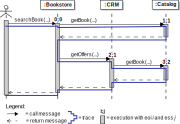
\includegraphics[width=0.96\columnwidth]{figures/eoiessBookstoreDemo-extended-2-combined}
\caption{UML Sequence Diagram illustrating our trace-related terminology}
\label{fig:exampleTraceTerminology}
\end{figure}

\begin{figure}\centering
% \vspace{-0.5cm}
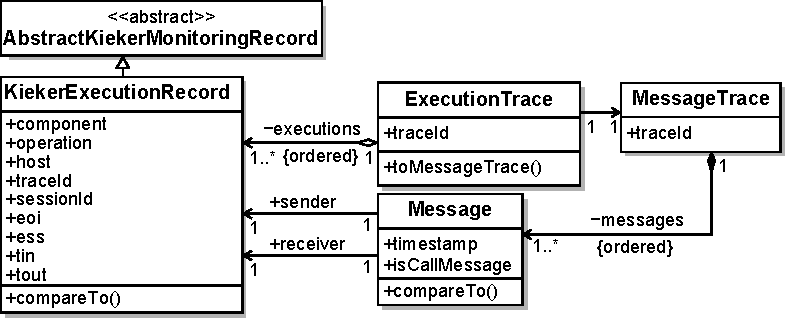
\includegraphics[width=1\columnwidth]{figures/kiekerTraceRepresentations-refined-bw}%
\caption{UML Class Diagram defining the trace-related information in Kieker.Tpan}
\label{fig:kiekerTraceRepresentations}
\end{figure}

\subsubsection{Logging Trace Information with \KiekerTpmon{}}

Kieker includes the \MonitoringRecord{} type \KiekerExecutionRecord{} which can %
be used to write \execution{} information into the \MonitoringLog{}. %
As shown in Figure~\ref{fig:kiekerTraceRepresentations}, an \KiekerExecutionRecord{} %
contains information about the executed \operation{}, the corresponding \component{}, 
the hostname on which the \execution{} was performed, as well as timestamps, %
typically with nanosecond resolution, for the start~(\textit{tin}) and end~(\textit{tout}) %
of an \execution{}. %
Kieker includes different \MonitoringProbe{} types for logging \KiekerExecutionRecords{} %
within an application, which look similar to the \MonitoringProbe{} in Listing~%
\ref{lst:aspectJRTMonitoringProbe}. %

A request to a system-provided service results in a nested control flow of %
corresponding \executions{}, referred to as a \textit{\trace{}}. %
Kieker provides efficient facilities for attaching a unique \traceIdentifier{} %
to the thread executing a service request, which is then contained in any %
\KiekerExecutionRecord{} of that \trace{}~(see~Figure~\ref{fig:kiekerTraceRepresentations}). 

\begin{lstlisting}[language=Java, float=*, numbers=none, xleftmargin=0pt,caption=Kieker.Tpan output of execution trace representation, label=lst:ExecutionRecordMonitoringLogExecutionTrace, basicstyle=\ttfamily\scriptsize]
TraceId 8430034814995791873 (NOSESSION):
<[0,0] 1257440666759412388-1257440666841265860 srv0::Bookstore.searchBook(..)>
<[1,1] 1257440666805601818-1257440666807695902 srv0::Catalog.getBook(..)>
<[2,1] 1257440666820790063-1257440666841169272 srv0::CRM.getOffers(..)>
<[3,2] 1257440666820839575-1257440666840922990 srv0::Catalog.getBook(..)>
\end{lstlisting}

%bin/tpan.sh -i /home/voorn/svn_work/pub_2009Kieker/tex-sources/tpmon-data/3_traceExample-tpmon-20091105-180426738/ -o tmp/ -p TSE --print-Execution-Trace
% \begin{lstlisting}[language=Java, float=*, numbers=none, xleftmargin=0pt, caption=Execution trace representation of trace~77, label=lst:ExecutionRecordMonitoringLogExecutionTrace, basicstyle=\ttfamily\small]
% <0 Bookstore.searchBook() .. 77 ..6759412388 ..6841265860 srv0 0 0 >
% <0 Catalog.getBook(boolean) .. 77 ..6805601818 ..6807695902 srv0 1 1 >
% <0 CRM.getOffers() .. 77 ..6820790063 ..6841169272 srv0 2 1 >
% <0 Catalog.getBook(boolean) .. 77 ..6820839575 ..6840922990 srv0 3 2 >
% \end{lstlisting}

%bin/tpan.sh -i /home/voorn/svn_work/pub_2009Kieker/tex-sources/tpmon-data/3_traceExample-tpmon-20091105-180426738/ -o tmp/ -p TSE --print-Message-Trace
% \begin{lstlisting}[language=Java, float=*, numbers=none, xleftmargin=0pt, caption=Message trace representation of trace~77, label=lst:ExecutionRecordMonitoringLogMessageTrace, basicstyle=\ttfamily\footnotesize]
% <..6759412388:$\$$|-send->Bookstore.searchBook()>
% <..6805601818:Bookstore|-send->Catalog.getBook(..)>
% <..6807695902:Catalog.getBook(..)|-return->Bookstore>
% <..6820790063:Bookstore|-send->CRM.getOffers()>
% <..6820839575:CRM|-send->Catalog.getBook(..)>
% <..6840922990:Catalog.getBook(..)|-return->CRM>
% <..6841169272:CRM.getOffers()|-return->Bookstore>
% <..6841265860:Bookstore.searchBook()|-return->$\$$>
% \end{lstlisting}
\begin{lstlisting}[language=Java, float=*, numbers=none, xleftmargin=0pt, caption=Kieker.Tpan output of message trace representation, label=lst:ExecutionRecordMonitoringLogMessageTrace, basicstyle=\ttfamily\scriptsize]
TraceId 8430034814995791873 (NOSESSION):
<SND 1257440666759412388 $\$$-->srv0::Bookstore.searchBook(..)[0,0]>
<SND 1257440666805601818 srv0::Bookstore.searchBook(..)[0,0]-->srv0::Catalog.getBook(..)[1,1]>
<RVC 1257440666807695902 srv0::Catalog.getBook(..)[1,1]-->srv0::Bookstore.searchBook(..)[0,0]>
<SND 1257440666820790063 srv0::Bookstore.searchBook(..)[0,0]-->srv0::CRM.getOffers(..)[2,1]>
<SND 1257440666820839575 srv0::CRM.getOffers(..)[2,1]-->srv0::Catalog.getBook(..)[3,2]>
<RVC 1257440666840922990 srv0::Catalog.getBook(..)[3,2]-->srv0::CRM.getOffers(..)[2,1]>
<RVC 1257440666841169272 srv0::CRM.getOffers(..)[2,1]-->srv0::Bookstore.searchBook(..)[0,0]>
<RVC 1257440666841265860 srv0::Bookstore.searchBook(..)[0,0]-->$\$$>
\end{lstlisting}

If the reconstruction of \traces{} from a \MonitoringLog{} containing \KiekerExecutionRecords{} %
would only include the \trace{} information presented so far, we would require the %
following assumptions: %
(a)~no two \execution{} start or end time events %
(\textit{tin}/\textit{tout}) within the same \trace{} occur at the same time; %
and (b)~clocks in a distributed system are perfectly synchronized (both with %
respect to the respective time resolution). %
Since both assumptions cannot be guaranteed in realistic environments, %
Kieker includes efficient facilities to attach two additional parameters to any %
\KiekerExecutionRecord{} in order to log the information needed to %
reconstruct (distributed)~\traces{} from the \MonitoringLog{} reliably: %
an \textit{\eoiLong{}~eoi} and an \textit{\essLong{}~ess}~(see~Figure~\ref{fig:kiekerTraceRepresentations}). %
\begin{description}
\item[eoi:] An \execution{} with an \eoiLong{} value~$i$ denotes the $i$-th %
\execution{} started within a \trace{} (starting with the value $0$).
\item[ess:] An \execution{} with an \essLong{} value~$j$ denotes an \execution{} that %
was started when the depth of the calling stack for the corresponding \trace{} was~$j$.
\end{description}

\noindent The \executions{} shown in the example \trace{} in Figure~\ref{fig:exampleTraceTerminology} 
are annotated with the corresponding \eoiLong{}~(eoi) and \essLong{}~(ess) values. %
Note, that while an \eoiLong{} is unique within a \trace{}, an \essLong{} %
value can, and usually does, occur more than once. %
% Listing~\ref{lst:ExecutionRecordMonitoringLog} shows the filesystem representation %
% of the \MonitoringLog{} for the example \trace{} of Figure~\ref{fig:exampleTraceTerminology}. %

\subsubsection{Trace Reconstruction with \KiekerTpan{}}

\begin{figure}\centering
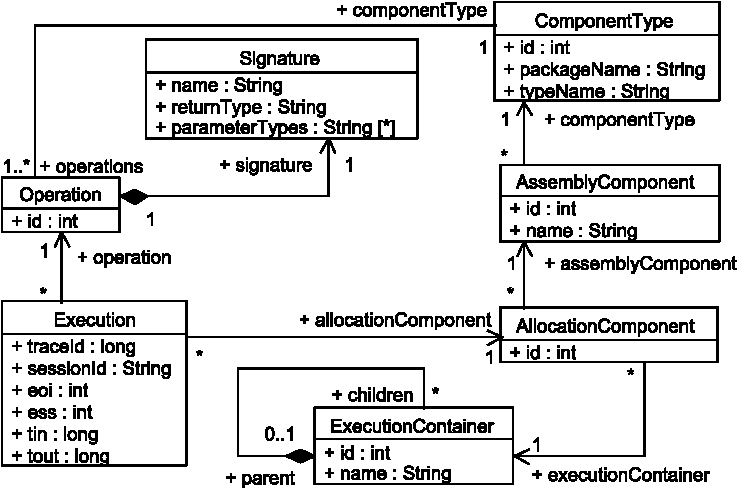
\includegraphics[scale=0.65]{figures/model/kieker_systemmodel-crop}
\end{figure}


In \KiekerTpan{}, two equivalent representations of \traces{} are used internally: %
\executionTraces{} and \messageTraces{}. %
An \executionTrace{} representation of a \trace{} is simply the ordered~(by %
\eoiLong{} values) sequence of \executions{}~(stored as \KiekerExecutionRecords{}, see Figure~\ref{fig:kiekerTraceRepresentations}). %
A~\messageTrace{} describes a \trace{} in terms of an ordered sequence of \Messages{} %
instead of \executions{}. %
Each \execution{} can be described by a corresponding \callMessage{}, %
representing an \operation{} call which starts the \execution{}, %
and a \returnMessage{}, representing the end of an \execution{} returning the %
control flow to the calling \execution{}, as illustrated in Figure~\ref{fig:exampleTraceTerminology}. %
For more details, refer to the associations \sender{} and \receiver{} in Figure~\ref{fig:kiekerTraceRepresentations}.
Listings~\ref{lst:ExecutionRecordMonitoringLogExecutionTrace} and \ref{lst:ExecutionRecordMonitoringLogMessageTrace} %
show text representations of the corresponding \executionTrace{} and a \messageTrace{} stored by \KiekerTpan{}, respectively.

Figure~\ref{fig:kiekerTraceRepresentations} shows the relations among \executions{}, %
\Messages{}, \executionTraces{}, and \messageTraces{}. %
While it is straightforward to derive \executionTraces{} from the \MonitoringLog{}, %
for later analysis it is usually easier to derive analysis models from \messageTraces{}. %
In \KiekerTpan{}, \executionTraces{} are derived from the \MonitoringLog{} and %
then transformed into equivalent \messageTrace{} representations from which %
analysis models and diagrams, as described in the following \mbox{Section~%
\ref{sec:traceAnalysisAndVisualization}}, are created.

% Underlying assumption: Each request is serviced by a trace of (nested) synchronous executions.

% In order to emphasize the caller/callee relationship among \components{} involved %
% in an \execution{} of an \operation{}, a message-oriented view can be taken by
% associating two types of \Messages{} with an \execution{}: %
% a \textit{\callMessage{}} and a \textit{\returnMessage{}}. %

% Implemented for distributed Web service scenarios (SOAP/cxf)

% \paragraph{From Execution Traces to Message Traces}\
% 
% Execution trace representation:
% \begin{itemize}
% \item Ordered set of executions (ordered by eoi)
% \item The monitoring log contains the unsorted executions
% \end{itemize}
% 
% Message trace representation:
% \begin{itemize}
% \item Ordered set of call/return messages
% \item Can easily be constructed from execution trace%\footnote{See {\scriptsize\texttt{kieker.loganalysis.datamodel.ExecutionTrace.toMessageTrace()}}\\}
% \item[$\rightarrow$] Straight-forward transformation to\\ sequence diagrams, dependency graphs, ...
% \end{itemize}
% 
% \TODOBOX{Show Algorithm}
% 
\subsection{Analysis and Visualization of Trace Information}\label{sec:traceAnalysisAndVisualization}

\noindent As described in the previous Section~\ref{sec:traceLoggingAndReconstruction}, %
\KiekerTpmon{} allows to log (distributed)~trace information to the \MonitoringLog{} %
which can then be transformed into two equivalent \trace{} representations using %
\KiekerTpan{}, i.e., \executionTraces{} and \messageTraces{}. %
These representations constitute the basis for \trace{}-based analysis and 
visualization functionality which can be integrated into the \KiekerTpan{} %
component. %
This section gives an overview of some of the \trace{}-based analysis and visualization %
functionality which have been integrated into \KiekerTpan{} so far: sequence diagrams, dynamic call trees, dependency diagrams, and Markov chains. %
By implementing a \MonitoringRecordConsumer{}, as described in Section~\ref{sec:architecture}, %
it is easy to implement custom components for analyzing and visualizing \trace{} %
information employing the Kieker framework.

%
% JPetStore dataset 3_20090710-163529-jpetstore-250Threads-400sDuration-200sRampup/
% 
% 236719 traces

\begin{figure}\centering
% bin/tpan.sh -i 3_20090710-163529-jpetstore-250Threads-400sDuration-200sRampup/tpmon-20090710-163529/ -p JPET --plot-Sequence-Diagram -o tmp/
% pic2plot -T svg tmp/JPETsequenceDiagram-19503.pic > tmp/JPETsequenceDiagram-19503.svg
% # removed package names in method signature w/ inkscape -> export to eps
% epstopdf sequenceDiagram-19503-noPackageName.eps
% \vspace{-0.3cm}
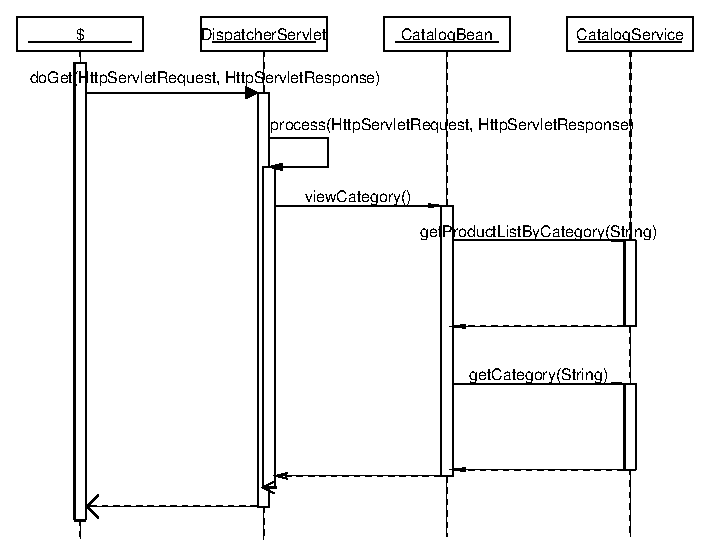
\includegraphics[width=\columnwidth]{figures/20090710-163529-jpetstore-250Threads-400sDuration-200sRampup-sequenceDiagram-19503}%
\caption{UML sequence diagram generated by Kieker.Tpan}
\label{fig:vis:jpetSeqDiagr}
\end{figure}

\subsubsection{UML~sequence diagrams}

UML~sequence diagrams provide a dynamic architectural viewpoint in terms %
of interactions among runtime objects implementing software services. %
In Figure~\ref{fig:exampleTraceTerminology} of the previous section, we used %
a sequence diagram to illustrate the \trace{}-related terminology needed to define %
\executionTraces{} and \messageTraces{}. %
\MessageTraces{} can be transformed to UML~sequence diagrams in a straightforward way. %
Figure~\ref{fig:vis:jpetSeqDiagr} shows such a UML sequence diagram generated by %
a Kieker visualization component for the iBATIS JPetStore which is a demo Java Web application implementing an
online store scenario.\footnote{The case study iBATIS JPetStore from \url{http://ibatis.apache.org/} is available as an instrumented version on the Kieker web page \url{http://kieker.sourceforge.net/}.} We employ this case study to give examples for visualizations in the present section. %
Given the timing information included in the \executionTraces{}, the sequence diagrams %
could easily be augmented with this additional data, e.g., observed response %
times. The UML~specification~\citep{OMG2007UML22Superstructure} and %
the UML~profiles for performance~\citep{OMG2005UMLProfileForSchedulabilityPerformanceAndTimeV1-1,OMG2008UMLProfileForMARTEBeta2} %
suggest appropriate notations for performance annotations. %
%Adding UML's combined fragments, e.g., loops and optional behavior, would only require %
%the definition of suitable \MonitoringRecords{} and corresponding \MonitoringProbes{} %
%collecting this information.\MR{Zum letzten Satz: Kann man loops etc. wirklich so einfach erkennen? Ich glaube da muss man mehr in der Analyse machen, wie soll das Monitoring einen Loop erkennen (Loop-Erkennung ist ein Problem fuer sich)... Besser den letzten Satz streichen, da wir es noch nicht bieten.}

\subsubsection{Dynamic call trees}

\begin{figure}\centering
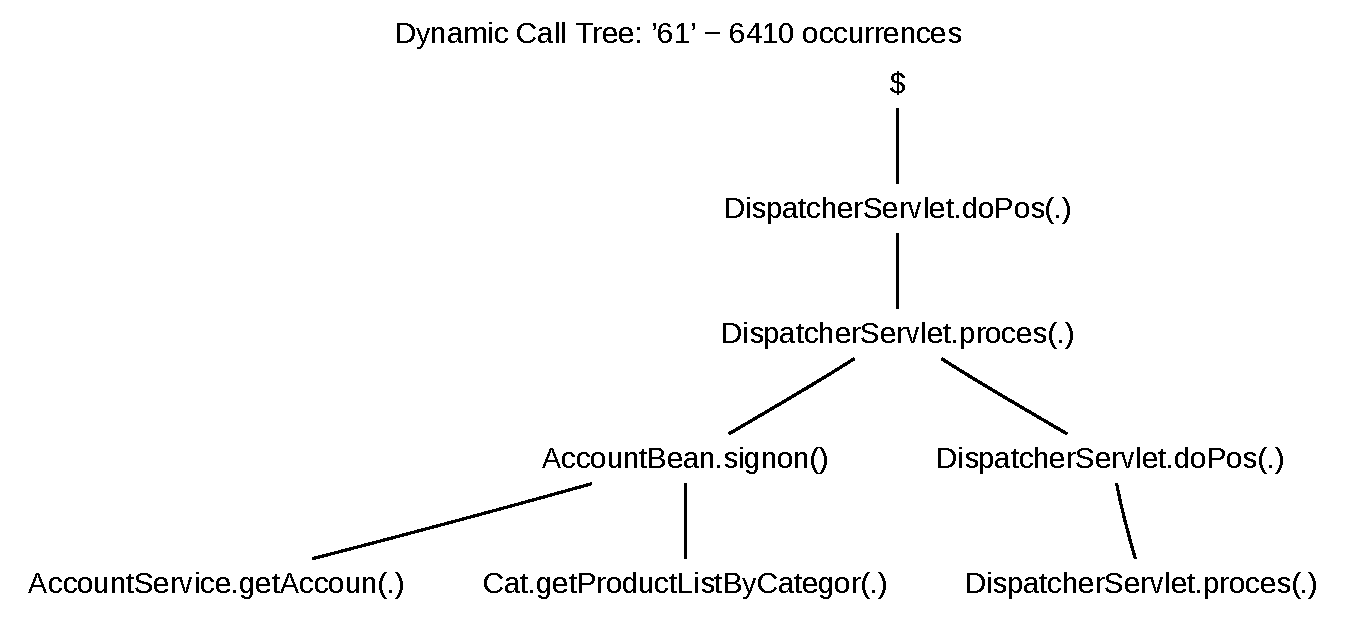
\includegraphics[width=\columnwidth]{figures/20090710-163529-jpetstore-250Threads-400sDuration-200sRampup-dynamicCallTree61}
\caption{Call tree corresponding to a trace equivalence class generated by Kieker.Tpan}
\label{fig:vis:jpetDepCallTree}
\end{figure}

Figure~\ref{fig:vis:jpetDepCallTree} shows an alternative representation of %
a \trace{}, called \textit{dynamic call tree}%
%\MR{Achtung! Habe `call tree' in `dynamic call tree' umbenannt (siehe Referenz AmmonsBallLarus97 S. 5)}
~\citep{AmmonsBallLarus97ExploitingHardwarePerformanceCountersWithFlowAndContextSensitiveProfiling}, generated by \KiekerTpan{}. A dynamic call tree %
contains the calling relations (\callMessages{}) among \operations{}, in contrast %
to a sequence diagram which also includes the corresponding \returnMessages{}. A dynamic call tree is an ordered graph, where the order (left to right) corresponds to the execution order of the nodes.
In~\citep{RohrvanHoornGieseckeMatevskaHasselbringAlekseev2008TraceContextSensitivePerformanceProfilingForEnterpriseSoftwareApplications}, %
we use the control flow information contained in a dynamic call tree to %
analyze the recorded response times of \operations{} based on the call tree position of the %
corresponding \executions{}.

When analyzing \traces{} from the \MonitoringLog{}, a valuable initial analysis %
is to determine the \trace{} \textit{equivalence classes}. %
Informally, a \trace{} equivalence class contains all \traces{} which are equal %
in terms of the control flow, i.e., the sequence diagrams of all \traces{} in an 
equivalence class are identical. %
Based on the \messageTraces{} this analysis can be implemented efficiently. %
Figure~\ref{fig:vis:jpetDepCallTree} shows the dynamic call tree common to all 6\,410~\traces{} %
in a \trace{} equivalence class extracted from the monitoring data of the JPetStore example. %

\subsubsection{Dependency graphs}

\begin{figure*}\centering
% bin/tpan.sh -i 3_20090710-163529-jpetstore-250Threads-400sDuration-200sRampup/tpmon-20090710-163529/ -p JPET --plot-Dependency-Graph -o tmp/
% dot -T eps tmp/JPETdependencyGraph.dot > tmp/JPETdependencyGraph.eps
% epstopdf tmp/JPETdependencyGraph.eps
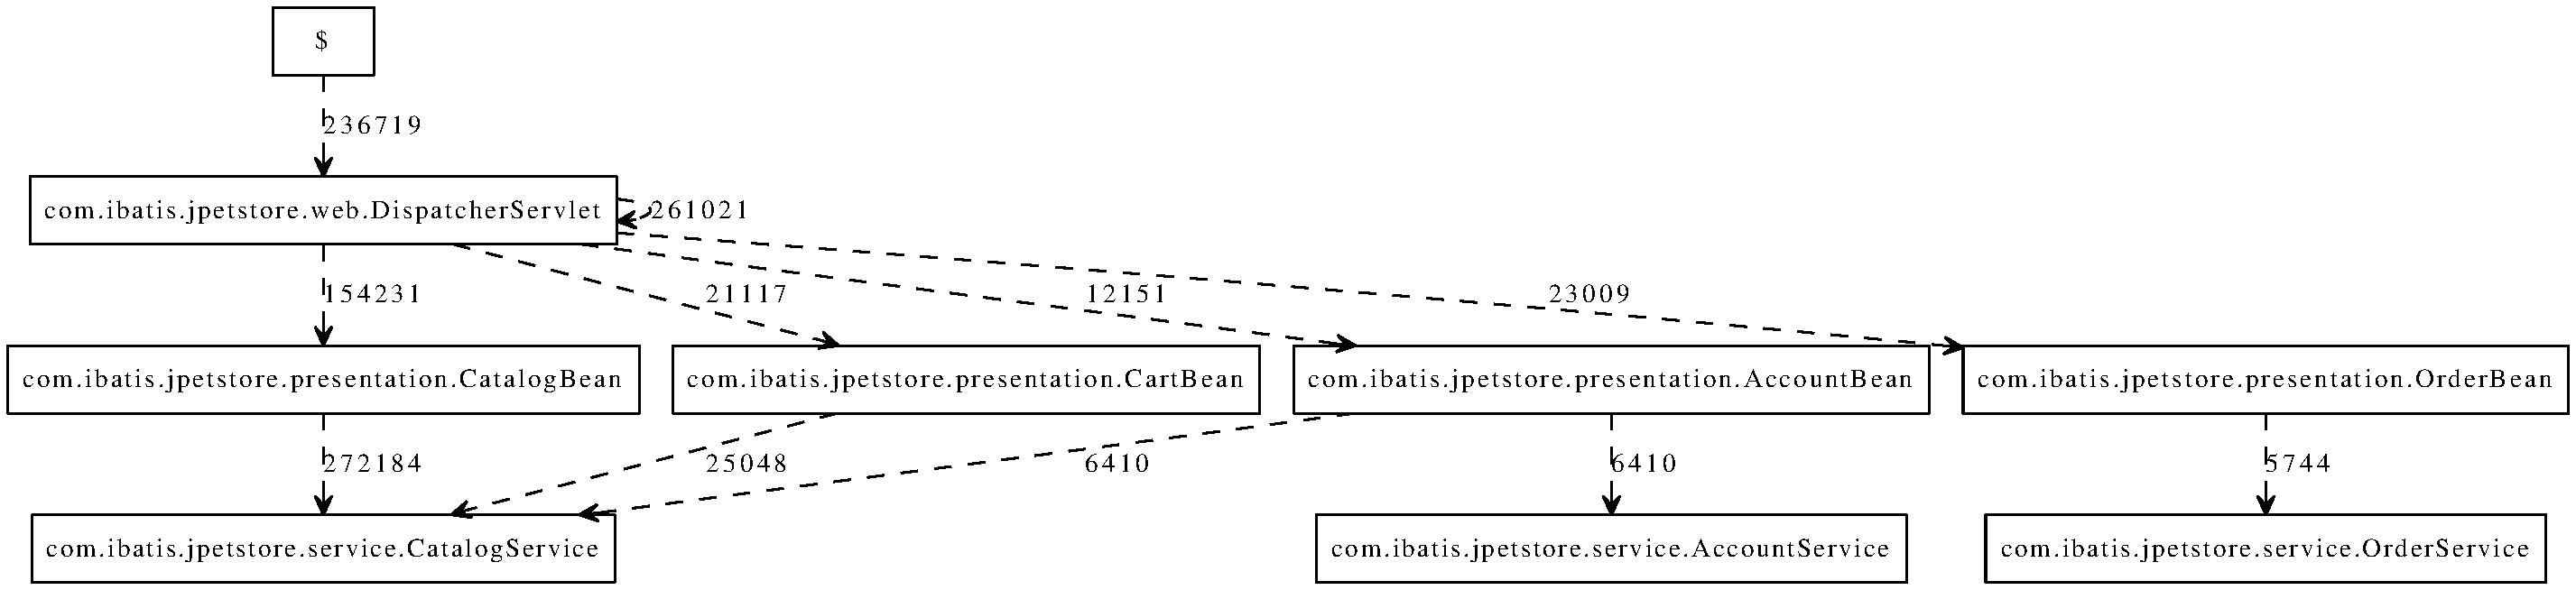
\includegraphics[width=\textwidth]{figures/20090710-163529-jpetstore-250Threads-400sDuration-200sRampup-dependencyGraph}%
\caption{Component dependency graph visualization generated by Kieker.Tpan}
\label{fig:vis:jpetDepDiagr}
\end{figure*}

While sequence diagrams, or \executionTraces{}, provide a view on the \textit{sequence} of %
interactions among objects in a single \trace{} (or scenario/use~case), it is often %
desirable to analyze this information in an aggregated %\MR{Ist es ganz klar ueber was man aggregiert?} 
form. %
Interactions among objects constitute runtime dependencies among these system %
entities, which can be described using weighted directed dependency graphs: %
each entity is assigned a node and each dependency relation %
an edge; the edge is directed from an entity using %(calling)
a particular service to the entity providing that service; 
the edges are augmented with the total number of call actions %\MR{actions statt messages? (UML)} 
among the respective entities observed in the considered set of \traces{}. %

We implemented a \KiekerTpan{} component which computes dependency graphs, %
% calling dependencies from \executionTraces{}, %
represented in adjacency matrices, from a set of \messageTraces{}. %
These dependency graphs are then available for further analysis or visualization. %
Figure~\ref{fig:vis:jpetDepDiagr} shows a dependency graph generated by %
\KiekerTpan{}, visualizing calling dependencies among classes of the partly-instrumented %
JPetStore application. The figure provides an aggregated view of the runtime dependencies %
observed in 236\,719~traces, resulting from 250~concurrent users simulated by probabilistic %
workload generation~\citep{vanHoornRohrHasselbring2008GeneratingProbabilisticAndIntensityVaryingWorkloadForWebBasedSoftwareSystems}. %

% In addition to dependencies among components~(or classes in this example), %
% \executionTraces{} allow to compute dependencies among execution contexts~(hosts) %
% and operations, which can then be represented as hierarchical dependency graphs. %
% Figure~\ref{fig:hierarchicalDependecyGraph} shows a drill-down view of a hierarchical %
% dependency graph, with weighted dependencies among deployment contexts, components, 
% and operations. The graph is augmented with failure diagnosis results based on 
% timing behavior analysis detailed in~\citep{MarwedeRohrHoornHasselbring2009AutomaticFailureDiagnosisInDistributedLargeScaleSoftwareSystemsBasedOnTimingBehaviorAnomalyCorrelation}.

\begin{figure}\centering
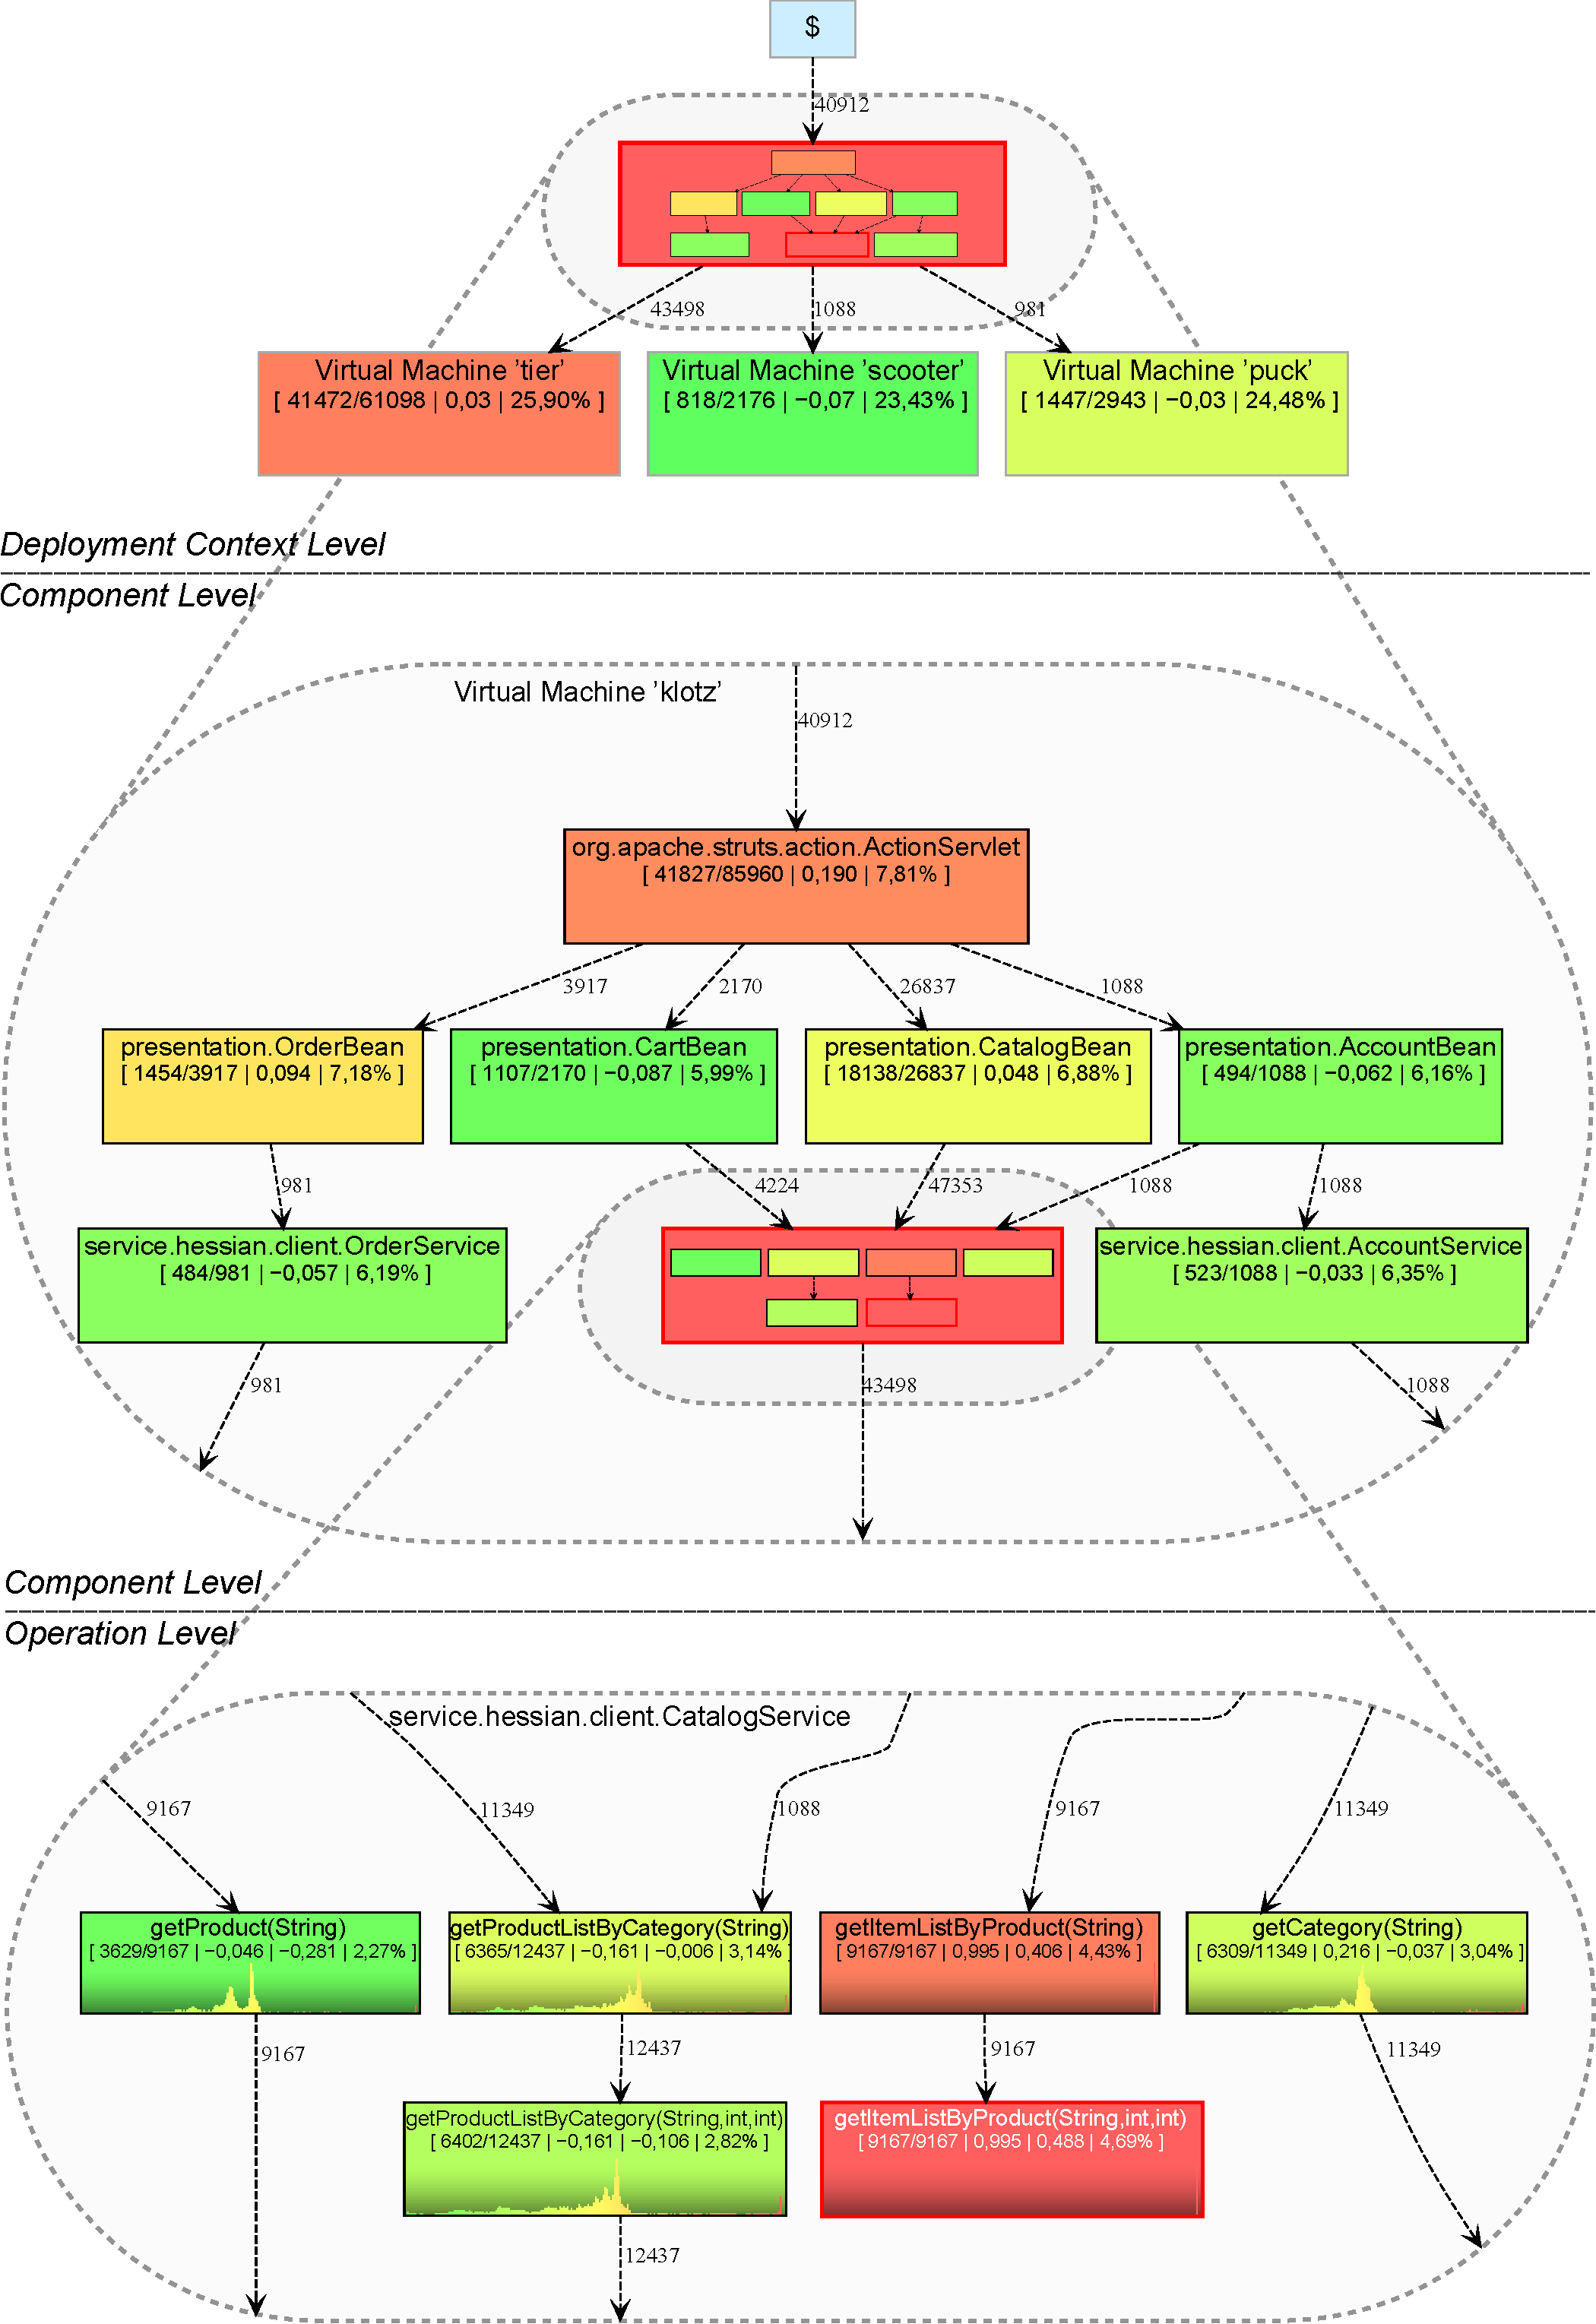
\includegraphics[width=\columnwidth]{figures/visualization-01}%
\caption{Visualized hierarchical dependency graph~\citep{MarwedeRohrHoornHasselbring2009AutomaticFailureDiagnosisInDistributedLargeScaleSoftwareSystemsBasedOnTimingBehaviorAnomalyCorrelation}}
\label{fig:hierarchicalDependecyGraph}
\end{figure}

Dependency graphs are employed by some approaches to runtime reconfiguration~\citep{SEAA07} or failure %
diagnosis~\citep{MarwedeRohrHoornHasselbring2009AutomaticFailureDiagnosisInDistributedLargeScaleSoftwareSystemsBasedOnTimingBehaviorAnomalyCorrelation}.
Figure~\ref{fig:hierarchicalDependecyGraph} shows a dependency graph that has been enhanced with anomaly score information to support failure diagnosis. %
In this visualization, three architectural levels (operation, component, and deployment context) are displayed and small histograms
show the distribution of the anomaly scores for each operation. Please refer to~%
\citep{MarwedeRohrHoornHasselbring2009AutomaticFailureDiagnosisInDistributedLargeScaleSoftwareSystemsBasedOnTimingBehaviorAnomalyCorrelation} for a detailed discussion; in the present paper this figure just serves as an illustration of possible visualizations.

% Software systems can be considered as a composition of communicating components. %
% Each component can provide some services while requiring external services. %
% A component A is dependent on component B, iff A uses/requires services provided %
% by B.  
% For illustration, %
% we extend UML component diagrams by including labeled dependencies~(see examples %
% in Figure~\ref{dependencyGraphsFigures}). The weight of an edge denotes the number %
% of actual requests for any service provided by the called component.
% 
% During runtime a system executes different scenarios and thus activates particular %
% instances of components. The runtime dependency graph among instances of components %
% at a particular point in time contains a subset of all possible dependencies of a %
% system. Considering the possibility of having a multi-user system, we can observe %
% a strong varying usage and thus varying dependencies among instances of components. %
% It is feasible to also determine the static dependency graph for the system as a %
% sum\TODO{/union?} graph from all possible execution scenarios. %Because of the problem of state explosion, we consider an experiment specific static dependency graph as a worst case runtime dependency graph for the monitored data.


% \TODOBOX{Andr\'e: Ab hier habe ich den Rest dieses Abschnitts noch
% cht \"uberarbeitet.}

% A widely used dynamic architectural viewpoint is given by UML sequence diagrams, %
% which allow to describe the interactions within object-oriented software systems. %
% A sequence diagram displays structural entities~(e.g., objects), their executions %
% (\textit{ExecutionSpecifications} in the UML) on the lifelines below them, as well %
% as call actions and returns between execution blocks.

% For this example, we partly instrumented a sample Web-based Java shopping system. %

% \begin{figure}\centering
% \includegraphics[width=0.48\textwidth]{figures/AddItemToCart2}%
% \caption{Sequence diagram}
% \label{fig:vis:seqDiagr}
% \end{figure}

% \begin{figure}\centering
% \includegraphics[width=0.48\textwidth]{figures/behaviorModel_buyer2-corrcted}%
% \caption{Markov chain}
% \label{fig:vis:markovChain}
% \end{figure}

% \begin{figure}\centering
% \includegraphics[width=0.48\textwidth]{figures/depDukeBankMockupGraph}%
% \caption{Component dependency graph}
% \label{fig:vis:dependencyGraph}
% \end{figure}

% \subsubsection{Markov chains}
% 
% \begin{figure}
%  \centering
% %trace id 3962531344010343978 database Andre table 070903_formula_fs_data
% %trace id 4148129190884353516 database Andre table 070903_formula_fs_data
% %the ``ItemSqlMapDao'' and other components with no connection were removed manually
% \includegraphics[width=0.9\columnwidth]{figures/MarkovChainBothTraces}
% \caption{Operation-level Markov chain for two message~traces~\citep{RohrHoornMatevskaStoeverSommerGieseckeHasselbring2008KiekerContinuousMonitoringAndOnDemandVisualizationOfJavaSoftwareBehavior}}
% \label{fig:vis:jpetDepMarkovChain} 
% %of the software system, generated from two Message traces that correspond to the two Sequence Diagrams
% %The states of the Markov chain represent the last message received within a particular trace and the edges point to messages that may be next with an expected probability larger than 0. The probabilities are learned from training data.
% \end{figure}
% 
% Markov chains are a common formalism used in reliability and performance theory~%
% (see e.g.~\citep{Trivedi2001ProbabilityAndStatisticsWithReliabilityQueueingAndComputerScienceApplications,MenasceAlmeidaDowdy2004PerformanceByDesignComputerCapacityPlanningByExample}) %
% to describe and analyze random processes, such as %computer 
% system and user behavior. %
% A discrete-time Markov chain describes a process in terms of a discrete number %
% of states and probabilistic transitions--in discrete time steps--among these. %
% The characteristic property of a Markov chain is that the next state of a process %
% solely depends on the process's current state. %
% An often used representation of Markov chains are (finite) state machines. %
% 
% % Markov chains provide a common stochastic means to describe dynamic system behavior %
% % of multiple scenarios. For example, Markov chains can, for instance, be used for intrusion detection %
% % to describe interactions among system components, and in reliability or performance %
% % analysis to characterize the utilization of components during service processing~\citep{GulSommerRohrVanHoornHasselbring2008EvaluationOfControlFlowTracesInSoftwareApplicationsForIntrusionDetection}. %
% % A (first order) Markov chain is a probabilistic %finite 
% % state machine with a dedicated entry and a dedicated exit state. Each transition %
% % is weighted with a probability. The sum of probabilities of outgoing transitions %
% % of a state must be $1$. Given the current state, the next state is randomly %
% % selected solely based on the probabilities associated with the outgoing transitions.
% 
% % \newpage
% 
% As illustrated in Figure~\ref{fig:vis:jpetDepMarkovChain}, Kieker can generate 
% finite state machine representations of Markov chains derived from a set of \executionTraces{}, %
% where the states represent the creation of a message within a \messageTrace{} and the edges %
% connect subsequent messages. The edges are labeled with the relative frequencies, %
% derived from the monitoring data, that messages follow each other. %
% A missing edge between two %
% messages expresses that the monitoring data analyzed contains no \trace{} with a %
% sub-sequence containing only these two messages. %
% Figure~\ref{fig:completeJpetstoreOperationProbabilityGraphAndMarkovChain} in Appendix~\ref{sec:appendix} shows %
% a single Markov chain generated from the 236\,719 traces of the JPetStore example. %
% 
% Our method used to compute Markov chains from \executionTraces{} is described %
% in~\citep{GulSommerRohrVanHoornHasselbring2008EvaluationOfControlFlowTracesInSoftwareApplicationsForIntrusionDetection}. %
% In that work, we present an application-level intrusion detection system by %
% comparing \executionTraces{} with normal behavior learned from monitoring data %
% and modeled as Markov chains. %

% %\clearpage


% At any time, the controller is in either of the following states: %
% enabled, disabled, or terminated. Transitions between these states can be %
% initiated externally by calling one of the coresponding methods, i.e., %
% \textit{disableMonitoring()}, \textit{enableMonitoring()}, and %
% \textit{terminateMonitoring()}. When the controller is not enabled, calls to %
% the method \textit{logMonitoringRecord(\dots)} have no effect and return %
% immediately. The meaning of the terminated state is that an unrecoverable error %
% occured and it is unsafe to proceed and the controller's state cannot be switched %
% to enabled or disabled any more. Arbitrarily frequent transitions between enabled %
% and disabled are possible in both directions, 

\clearpage

\appendix

\section{Kieker Architecture}

At the 2010/03 Kieker Developer Meeting at University of Kiel the target Architecture for the next major releases of Kieker was defined. The architecture is outlined in Figures~\ref{OverviewArchitecture201003} and \ref{DetailedArchitecture201003}.

\begin{figure}
 \centering
 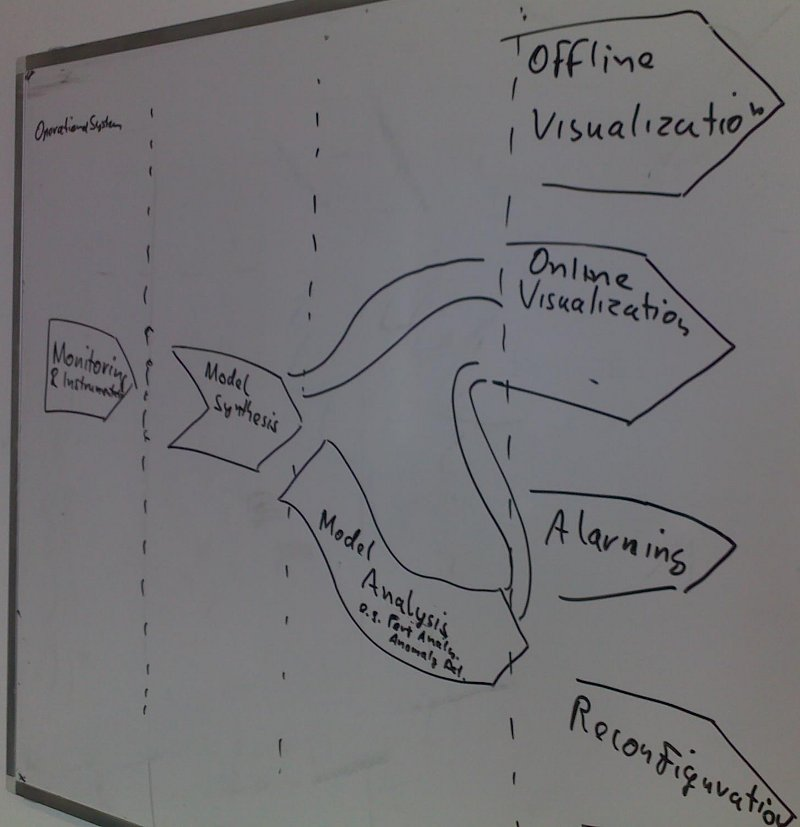
\includegraphics[width=0.4\textwidth]{./figures/2010-03-09-TargetArchitectureOverview.jpg}
 % 2010-03-09-TargetArchitectureOverview.jpg: 800x827 pixel, 72dpi, 28.22x29.17 cm, bb=0 0 800 827
 \caption{Overview of the underlying design principle for the Kieker architecture.}\label{OverviewArchitecture201003}
\end{figure}

\begin{figure*}
 \centering
 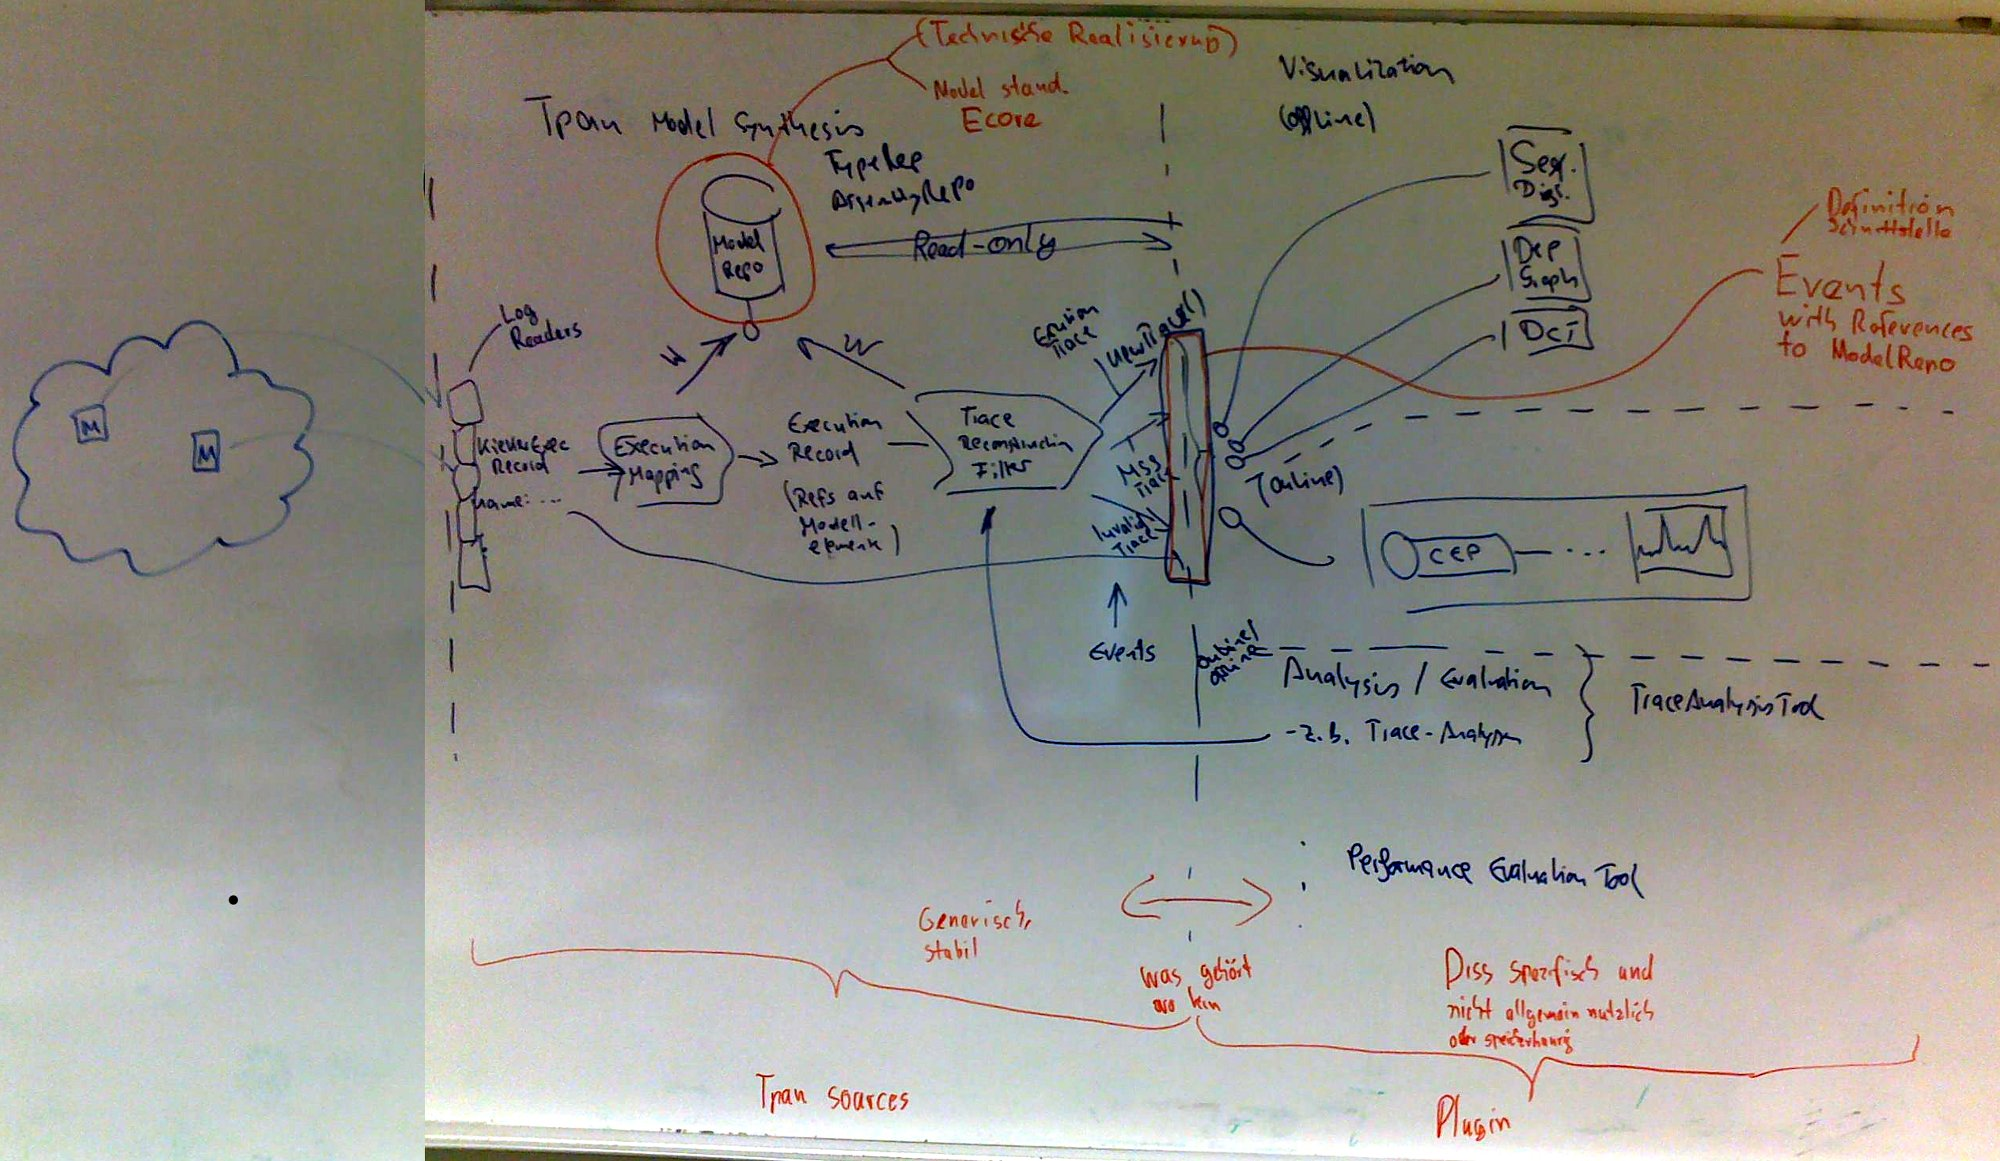
\includegraphics[width=0.9\textwidth]{./figures/2010-03-09-TargetArchitectureDetail.jpg}
 % 2010-03-09-TargetArchitectureDetail.jpg: 2000x1161 pixel, 72dpi, 70.56x40.96 cm, bb=0 0 2000 1161
 \caption{Detailed Kieker Target Architecture}\label{DetailedArchitecture201003}
\end{figure*}

Basic architectural principles are:
\begin{itemize}
 \item Event driven architecture with several publish/subscribe layers.
 \item Tpan has a common set of event publishers that refer to model objects that are in the ``model repository''. These common objects are for instance traces, operations, messages.
\end{itemize}



\nocite{vanHoornRohrHasselbringWallerEhlersFreyKieselhorst2009TRContinuousMonitoringOfSoftwareServicesDesignAndApplicationOfTheKiekerFramework,RohrHoornMatevskaStoeverSommerGieseckeHasselbring2008KiekerContinuousMonitoringAndOnDemandVisualizationOfJavaSoftwareBehavior}
\bibliographystyle{unsrtnat-abbrv} %abbrvnat, abbrvnatAvanhoorn % alpha
\bibliography{bibliography}

\end{document}
